\setlength{\parindent}{0em}
\setlength{\parskip}{1em}
\chapter{Introduction}

Linux distributions are build upon packages which provide software to their users. It is these
packages that make particular distribution different or similar to other one. All these packages require
maintenance, in the case the distribution is developed commercially, as well as it is developed by community.
The fact that the whole system is stable and comfortable to use is a result of a good work of
maintainers who work together to ensure that all packages are working and their
requirements are met.

An efficient maintenance requires accurate information which maintainers get from multiple sources
and are using many tools to retrieve. For example, which packages depend on their own packages and thus which
maintainers should they communicate with when encountering disturbing changes. Often the information
is not easy to acquire and slows down developers by forcing them to manually search through different
places. To solve this problem a new tool which is able to store and filter any information about
packages is required as no other exist in the moment of making this thesis.

RPQR is an originally proposed tool which is supposed to make maintainers life easier by allowing them to describe how
to acquire the data only once and then being able to retrieve it on demand. It is flexible
enough to store any new kind of data and to search packages based on combination of any of them while
also providing the option to accelerate queries by making specialized commands.
RPQR also lets users build a cache which makes further queries faster and thus saves time while
doing everyday work.

the tool is able to be directly used by other projects through provided API or it can be used
by user as any other command line project. Users are also able to visualize their
results for faster understanding of the results.

\chapter{Theory and current state}
While crucial information about a RPM package is stored directly inside it within the header section,
additional information as who maintains it or which bugs are currently known has to be searched
in external sources of information. This chapter describes RPM packages and technologies which
currently exist for working with them. Then we continue with a description of other subjects which are needed
to successfully design and implement RPQR project.

\section{RPM package}
RPM packages have their own file format\cite{RPMFileFormat}. It is composed of four parts with their specific purposes.
The parts are (i)lead, (ii)signature, (iii)header and (iv)archive. Here are described and explained all parts
relevant to the RPQR project.

\subsection*{The lead}
The lead is the first part of the RPM package. It contains magic number and version of RPM file format.
It also contains whether the package type is binary or source and other information relevant
for system using it. The difference between binary and source package is that source package contains
source code from which software can be built or the whole downloaded project, while binary package
contains the actual software. The lead is no longer used internally by RPM because of its
inflexibility and is noted here only for completeness of file format description.

\subsection*{The signature}
The signature is allowing package integrity and optionally authenticity to be verified. It holds
little purpose for RPQR but it is important because dnf uses it and RPQR is using dnf API.

\subsection*{The header}
The header is the most interesting part from perspective of RPQR project, because it contains
detailed crucial information about the package. It is composed of tags which describe different
aspects of the bundled software. Examples of these tags can be \mbox{\textit{RPMTAG\_VERSION}}
specifying version of the package or \textit{RPMTAG\_RELEASE} which specifies what release of
this version this is. Header is parsed by a software which is making metadata structure of RPM
repositories and this structure is then used by the dnf package manager to find appropriate
packages that the user needs.

\begin{lstlisting}
00001198  8e ad e8 01 00 00 00 00  00 00 00 3e 00 00 0f dd  |...........>....|
\end{lstlisting}

The first 16 bytes of header part are describing attributes of this header. Three bytes are
magic number identifying header, one byte says that header conforms to version 1 of specification.
Four another bytes are reserved and then there is count of entries stored in this header
(00 00 00 3e to decimal is 62). The last four bytes mean how many bytes is stored in this structure
(00 00 0f dd to decimal is 4061).

\begin{lstlisting}
000011c8  00 00 03 e8 00 00 00 06  00 00 00 02 00 00 00 01  |................|
\end{lstlisting}

For best example, we will describe name tag. 00 00 03 e8 identifies presence of
name tag and 00 00 00 06 says that value is string. 00 00 00 02 means that value
is located 2 bytes after the start of store and 00 00 00 01 indicates that there is
just one value, which is the only allowed possibility for string value stored in the header.

The store is just values after each other and are distinguished only by their respective offsets.

\subsection*{The archive}
The archive is a set of files and folders compressed with gzip compression algorithm. Its integrity
can be verified with signature specified.

\section{RPM repository}
RPM repositories are directory structures which contain RPM packages and metadata which are needed
to quickly locate packages that user needs. Metadata are created by createrepo \cite{RPMRepository}
utility and accessed by dnf package manager. 

\subsection*{Repodata}
Every RPM repository contains folder \textit{repodata} which contains data about contents of the
repository. There is a file \textit{repomd.xml} containing xml structure indicating where should
package manager look for databases with information about packages.

Important databases:
\begin{itemize}
  \item \textbf{primary} database which specifies all crucial information about each package as version, description or file list.
  \item \textbf{other} database which contains other less important information e.g. changelog of a package
\end{itemize}

\section{Package managers}
Work with RPM packages can be done by multiple tools. Their general responsibility is to recognize
package dependencies and being able to install or uninstall software contained in the package.
Most frequently used are RPM package manager and DNF package manager (successor of the old
YUM package manager).

\subsection*{RPM package manager}
RPM package manager supports more low level operations with packages than DNF does \cite{RPMPackageManager}. It allows
to build source of a project according to specfile and create distributable packages. More of the
important operations are also reading of the metadata and verification of installed software, in
case that it is not working properly. Installation of dependencies would have to be handled by user
manually so rpm utility is not often used by end users of the systems.

\subsection*{YUM package manager}
Yum package manager is historically the first manager that allowed easy downloading of packages
from remote repositories and handling their dependencies \cite{YUMPackageManager}. It is currently deprecated and has been
replaced by DNF. Reasons for deprecation and replacement were that YUM was not properly documented,
it was not ready for switch to python3 and algorithm for dependency resolvement was not strong enough
to handle all problems that withstand in modern RPM based linux distributions.

\subsection*{DNF package manager}
DNF package manager is a successor of the older YUM package manager \cite{DNFPackageManager}. It allows user to install and remove software
on system comfortably by handling all of the operations that are needed to retrieve package dependencies
and resolve any of the possible conflicts. Very often used feature is also system upgrades, when
DNF is able to migrate system from old versions of distribution to new ones. Very important fact
that needs to be stated is that DNF provides python API which can be used by other projects to retrieve metadata
from repositories and distinguish them.

DNF is the only tool that is currently able to query repositories for metadata which are specified
in packages. An example of frequently used query is:

\textit{\$ dnf repoquery --whatprovides /usr/bin/bash}

This command issues that dnf should execute command repoquery filtering by tag \mbox{\textit{provides}}
and find all packages that provide file \textit{/usr/bin/bash}. DNF is able to search for packages based by
attributes which are supplied within the package, but it is not able to retrieve additional information
or query based on complex relationships. It is not its job to resolve more difficult queries and
it would be wrong to force it to by extending its capabilities.

\section{DNF API}
DNF provides python API through which developer can interact with repositories and retrieve information.
At first instance of \textit{Base} class has to be created and then specify repositories from which
metadata should be retrieved. Call to \textit{fill\_sack} method after that will load the metadata
and API can then execute queries which the dnf tool supports.

Example of how is dnf API used in RPQR project:
\begin{lstlisting}
  base = dnf.Base()
  for (name, url) in self.repositories:
      base.repos.add_new_repo(name, base.conf, baseurl=[url])
  base.fill_sack(load_system_repo=False, load_available_repos=True)
  return base.sack.query().available()
\end{lstlisting}

\section{Storing techniques and query language}
As was stated before, it is crucial to choose the right technologies to store package metadata in
such a format that they can be read by human reader while also easily parsable and serializable.
This section will describe possible formats. Another part will be explaining existing query
languages which could be used for RPQR queries and their pros and cons in context of describing
package metadata.

\subsection*{Data structures}
While RPM repositories store metadata as a list in XML format or sqlite database, for use cases that
are oriented about relationships between packages list does not have to be appropriate data
structure for internal representation of package metadata.

\begin{itemize}
  \item List
    \subitem Pros:
    \subsubitem Easy to work with Python
    \subsubitem Simple algorithms to process its members
    \subitem Cons:
    \subsubitem Bad handling of relationship representation
  \item Dictionary
    \subitem Pros:
    \subsubitem Faster accessing of members
    \subitem Cons:
    \subsubitem Forcing packages to be identified by the same attribute
  \item Graph
    \subitem Pros:
    \subsubitem Great representation of relationships between packages
    \subsubitem Fast algorithms for searching and filtration
    \subitem Cons:
    \subsubitem More complex algorithms for processing of nodes
    \subsubitem To filter packages according to attributes, dictionary or list is still needed
                since there is no package that we could consider as proper root of the graph.
\end{itemize}

\subsection*{Data formats}
Appropriate data format needs to be chosen for storing of data. Currently there are many massively
used formats which could be suitable for RPQR use case. Data format should be chosen accordingly to
how much readability it can provide for human developer and whether it can used within versioning
repositories such as git or mercury.

\subsubsection*{XML}
Extensible markup language\cite{XMLFormat} is used by repocreate utility which is parsing package metadata and creating
their collections for package managers. It is natively supported by Python and relatively easy to
read. XML is using tags to distinguish individual elements of serialized data. Its advantage
is that it supports various encodings and even can contain comments so some things in serialized
data could have additional explanations when needed.

Example of XML data:
\begin{lstlisting}
  <?xml version="1.0" encoding="UTF-8"?>
  <element>
      <innerElement>
        Example text
      </innerElement>
      <!-- Explanation comment -->
  </element>
\end{lstlisting}

\subsubsection*{JSON}
JavaScript Object Notation\cite{JSONFormat} is widely used format for data serialization which represents objects
with pairs of named attributes and their values. One of the big advantages is that it also natively
supports arrays and consists of minimal syntax which allows most data to be stored and transferred
with less required space. Unfortunately there is no support for comments but readability of JSON
data is generally good so they are not needed in most cases.

Example of JSON data:
\begin{lstlisting}
  {"Element":{
    "InnerElement": "Example text"
    }
  }
\end{lstlisting}

\subsubsection*{YAML}
YAML\cite{YAMLFormat} Ain't Markup Language is data format used by many applications for configuration and data
transfer. YAML used JSON as a basis for its version 1.2 and it is accepting JSON as its subset.
Interesting about this format is that unlike JSON it supports comments and extensible data types.
Strings in YAML can be also specified without the starting and ending quotation marks. Individual
attributes of objects distinguished by name and indentation style similar to Python. While
YAML data sets are generally smaller than JSON, the number of additional syntax features makes
their parsers more complex and thus it inevitably takes more time to load them.
\newpage

Example of YAML data:
\begin{lstlisting}
element:
  InnerElement: Example text
\end{lstlisting}

\subsubsection*{Pickle}
For completeness here is mentioned even Python pickle format\cite{PickleFormat} for object serialization. Because
it is binary it can be parsed more quickly and support additional acceleration of RPQR execution.
There is an issue with execution of arbitrary code when parsing pickle structures which does not
occur in previously mentioned formats. Unlike the previous formats, it is not human readable
and thus unfortunately not appropriate to be used for package data structures that should be accessible
by different tools.
There is not an example because it would not make sense to show binary data.

\subsection*{Query languages}
For purposes of RPQR project, there needs to be a specification how to describe queries. Currently
there are many approaches. In this section there will be description of some of them and their features
which could prove useful for selecting packages and their attributes.

\subsubsection*{SQL}
Structured Query Language\cite{SQL} is a domain-specific language which is widely used to interaction with
relation databases. SQL is able to select records based upon their attributes and relations but
is not capable of describing complex recursive queries about graphs. Another caveat is that for Python
application, using standard Python libraries, to be able to use SQL, it would need to hold an instance of sqlite database in memory and
that could prove to be unnecessary overhead which could slow execution down.

Example of SQL query:
\textit{SELECT * FROM table WHERE id = 3}

\subsubsection*{GraphQL}
GraphQL\cite{GraphQL} is an open source query language which allows developers to implement their own interpretation
of individual query parameters. It is used in REST APIs to allow client applications to retrieve data
effectively from a server without it having to transfer any unnecessary data. Its flexibility is
a great advantage but queries are not as readable as they would be in SQL language.

\subsection*{Cypher query language}
Cypher query language is an implementation of opencypher specification. It is meant for work with
neo4j graph database and is developed for such purpose. For application to be able to get advantage
of cypher, it needs to use neo4j database which can result in too big an overhead for utilites
designed with one specific purpose in mind.

Example of Cypher query language:

\textit{MATCH (peter: employee {name: 'Peter Parker'}) RETURN peter}

\newpage

Example of GraphQL query:

\begin{lstlisting}
  {
    table(where: {id: {_eq: 3}}) {
      id
      name
      age
    }
  }
\end{lstlisting}

\subsubsection*{Domain specific language on Python}
Creating own query language is always and option and it holds enormous power in the ability to
bend the language to the specific purpose that RPQR project needs. Problem is that developing
and maintaining language takes time and energy. For a language to be functional, RPQR would
need to implement its own components like scanner, parser and interpreter. In the essence,
domain specific language for RPQR would need to be relatively simple. There is a requirement
to interpret statements which result is always set of nodes that represent packages. These
statements consists of commands that take values and other statements as arguments and operators
which realize basic set operations as is union or intersection.

Example of how RPQR language could look:

WHATDEPENDSON('libyang', 3) \& WHATDEPENDSON('libgcc', 3)


Components that are needed for interpretation of RPQR language:
\begin{itemize}
  \item \textbf{Scanner}

  Scanner is used to convert source text of the language to tokens for further processing by parser.
  Its crucial part is finite state machine which reacts to characters in input and recognizes lexical
  tokens. Scanner is also able to tell user when some lexical error occurs and query needs to be
  changed for it to be valid.
  
  \item \textbf{Parser}
  
  Parser consumes tokens from scanner and handles creation of abstract syntactic tree or some other
  internal representation of source text on input. Parser is able to recognize syntactic errors
  which occur during parsing and optionally inform user about them. There are multiple techniques
  for syntactic analysis as Top-Down Parsing or Bottom-Up Parsing which are basically algorithms
  how to recognize language unit on input. Both of these techniques are using models for context-less
  languages such as formal grammatics. Formal grammatic is a list of rules which are used to check
  whether input is written in a language or not.
\newpage

  \item \textbf{Interpreter}
  
  RPQR does not need to translate query into some other form, it needs to perform it. That is the
  reason why last part of RPQR language would be its interpreter. Interpreter inside of RPQR would need to be
  flexible enough for it to be able to accept new commands for searching of packages. Another thing
  that is important is using optimizations such as short evaluation to make searching of packages
  as fast as possible.
\end{itemize}

\section{Caching}
Since one of the most time consuming actions of current approach to queries about RPM packages is
network communication and transfer of metadata, it is crucial to download all metadata at once on
the start of execution to not need any further downloads. This can be ensured through DNF API by
executing query to list all packages that are available to install from specified repositories.
DNF package manager uses very similar approach by downloading all metadata to local storage and
updating it only when user forces it to or cache expires.

Question of metadata expiration needs to be handled by RPQR itself too.

Approach when metadata are not updated unless user wants to do so could save time for
checking of repository but user would be responsible for consistency of metadata and repository
state which could prove problematic.

RPQR could stick with the same approach as the DNF one. Rebuild metadata when they expire.
The problem is that building internal structure and rebuilding cache could be very time consuming
operation maybe even in the matter of minutes.

The third and maybe the most proper approach is to set expiration time of metadata to some
longer period of time. After such period the time for rebuilding of cache will not be so important.
Also if no change occured then it is pointless to rebuild the data and it would be highly useful
to rebuild only parts of internal data structures which do not longer correspond with the actual state
of RPM repositories supplied in configuration.

\section{Configuration}
It is clear that the RPQR tool will need multiple options for it to work properly and accordingly to
users notions. There are multiple ways how to supply such configuration to the tool. One of the
most common ones is to supply configuration by command line options. While this is easy to implement
and Python offers native support for it, this approach could prove to be painful for user when
overused. For example six or more commandline options would be difficult to track. That can be solved
by providing user with means to set mostly static options through configuration file.

\newpage

With configuration file withstands more choices which needs to be done.
\begin{itemize}
  \item Format of the configuration file
        There are multiple formats which can be used. JSON or YAML are probably the most appropriate ones.
        Their description was stated in previous sections.
  \item What options should configuration include
        Configuration should include only options which does not change often and thus do not force
        user to change the file frequently.
\end{itemize}

\chapter{Research}
With good knowledge about current state of utilities and technologies, this chapter can explore
what is the best approach to resolving complex queries about RPM packages. In each section
there is described particular approach that was choosen as a best for solution of individual problem.

\section{Project structure}
Python project is most often divided into folders which contain logically related classes
and classes that have less dependencies are located deeper in a directory structure. So entire
implementation of projects logic has one root folder. Another folder is meant for executble
binaries or scripts that are supposed to be installed in path of users system. The last important
folder is folder containing tests. There is multiple ways to store projects test but own folder
seems to be most clean and tests seeking utilities have easier time to find tests organized in
such way.

Illustration of proposed structure:

\begin{lstlisting}
bin
bin/script
project
project/example\_module
test
test/example\_module
\end{lstlisting}

\section{Retrieval of information from repository}
While there are approaches which would allow individual retrieval of metadata from repositories,
such as custom downloading of xmls and database archives, there is no reason for that, because
DNF provides API that allows application to use its already implemented downloading of metadata.
The best way to use it for this purpose is to create query which matches with every package
accessible through configured repositories.

\section{Customization and modyfication of functionalities}
RPQR project needs to be able to adapt to changing demands on queries and the most simple way to
achieve that is to create a system of loading plugins in a form of python modules. There is no
out of the possibility for Python script to dynamically load another module but because of a very
high level of introspection that Python provides, it is possible to achieve something very simmilar.
When plugin upholds certain defined rules, such as that class for load is named the same as the file,
then it is possible to easily create efficient algorithm for searching and importing of accessible
plugins.

Illustration of plugin importing:
\begin{itemize}
  \item Gather all directories for inspection from configuration or use hard coded paths
  \item For each folder walk over files and check if they fulfill naming rules
  \item Try to import classes by names devised from file names
\end{itemize}

Naming conventions for files containing plugins:
\begin{itemize}
  \item File name can not start with underscore (Python uses \_\_init\_\_ files
  in directories and we need to omit them, also there has to be a possibility to add supplementary files without importing them)
  \item Class that should be imported has to have the same name as the file (this way we can avoid
  implementing unnecessary overhead by looking through the module and searching for class by some
  more rules)
\end{itemize}

Plugin will contain one main class that can define how to retrieve data that it needs and commands
that can be used to filter packages by this attribute or relationship. Enforcing of good structure
will be done by providing base classes which plugins need to extend.

\section{Internal structure of data representation}
For RPQR to be able to effectively walk through packages and filter them by attributes and relationships
, there has to be appropriate way to access them as quickly as possible. That is why by nauture, graph
is the best way. Using graph will allow RPQR project to use graph algorithms such as breadth first search
or depth first search. Python itself does not have builtin graph support, so RPQR project can either
contain its own implementation or use a library.

Networkx seems to be very quick and easy to use implementation of graph abstract data type which is
also capable of rendering a graph with multiple algorithms when needed. Another very useful feature
is that networkx is able to save graph to JSON formatted string and load it again from this string.

Example of building graph with Networkx:
\begin{lstlisting}
  import networkx as netx
  graph = netx.Graph()
  graph.add_node(1)
  graph.add_node(2)
  graph.add_edge(1,2)
\end{lstlisting}

\section*{Configuration}
Some options are uncomfortable to enter through commandline repeatedly and because of that should
be stored in persistent file. Structure of configuration file can have many forms but Python has
built-in module named configparser which defines human readable format appropriate for RPQR project.
Configparser uses section to divide configuration into logically related blocks, there will be
main section for global options like urls of repositories. Each plugin will have its own section
where it will be possible to disable it or provide individual information neccessary for its proper
function.

Example of configparser configuration file:
\begin{lstlisting}
[first_section]
option1 = 1
option3 = filepath
[second_section]
option2 = 2
\end{lstlisting}

\section{Query language design}
RQPR language is by nature of its use oriented on filtering sets and thus will constructed from
statements and operations between them. This section will thoroughly describe the language and
its formal description from the view of formal language theory.

\subsection*{Lexical analysis}
RPQR will use finite state machine for scanning of tokens present in entered query and putting them
in list that can be further processed. Each of the lexical tokens is defined by regular expression
and when not recognized can be marked as invalid.

Finite state machine graph:

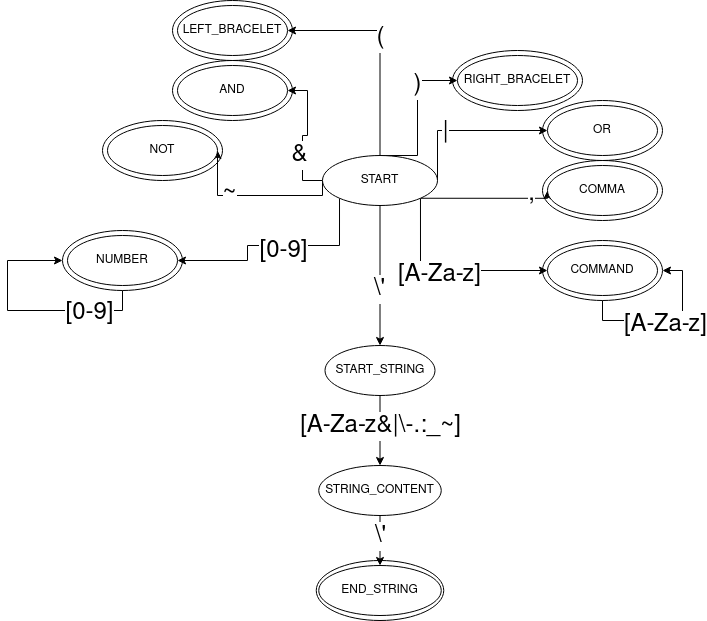
\includegraphics[scale=0.5]{obrazky-figures/RPQR_FSM.png}

The lexical tokens that occure in RPQR language are:
\begin{itemize}
  \item left bracelet (
  \item right bracelet )
  \item and operator \&
  \item or operator |
  \item negation operator ~
  \item number (consisting only of numeric characters e.g 123)
  \item string (hyphen separated string of alphanumeric and special characters e.g 'hello')
  \item command (command contains only alpha characters and has to be described by a plugin e.g NAMELIKE)
  \item comma used mainly as a separator for command arguments ,
\end{itemize}

\subsection*{Syntactic analysis}
RPQR language syntactic analysis will be mainly precedent syntactic analysis because the language is statement
oriented. Precedent syntactic analysis uses algorithm with symbol stack and acts accordingly to precedent
syntactic table. This table defines what operators can be used at particular places and their respective
priorities. This solves the problem of evaluation of statement but there is still the matter of command
recognition and validation of argument types. Every command has to define what arguments it needs to work
properly. Initial configuration of RPQR will load commands and create context less gramatic for them.
Because every command has different name and there is no need for dynamic arguments, distinction should
be straightforward and effective.

Another more problematic matter is that for RPQR language to be able to handle all neccessary use cases,
commands need to be able to accept results of other commands as arguments. This is problematic, since
it requires new instance of precedent syntactic analysis to parse this statement. Fortunately this
can be solved by cutting substatement out of original statement and putting it queue of statements
that have to be yet parsed.

After all these problems are solved, RPQR will have abstract syntactic tree containing all the information
that is neccessary for exectution of statement e.g. commands that need to be executed first and operators
located in depth accordingly to their precendence. This tree will be later processed by semantic
analysis e.g. interpreter.

Precedent syntactic table used for RPQR language:

\begin{center}
  \begin{tabular}{ |c|c|c|c|c|c|c| }
   \hline
     & ( & ) & \& & | & \textasciitilde & \$ \\
     \hline
  (  & < & = & <  & <  & <  & \#  \\
  \hline
  )  & \# & > & >  & >  & >  & >  \\  
  \hline
  \& & < & > & >  & <  & <  & >  \\
  \hline
  |  & < & > & <  & >  & <  & >  \\
  \hline
  \textasciitilde  & < & > & >  & >  & <  & >  \\
  \hline
  \$ & < & \# & <  & <  & <  & X \\
  \hline
  \end{tabular}
\end{center}

\textbf{Explanation of symbols}

Algorithm which handles syntactic analysis is driven by the precedent syntactic table. It always
looks at the first terminal symbol at the top of the stack and performs operation that is specified
in table by what symbol is in input.
\begin{itemize}
  \item < means that special symbol marking start of particular statement needs to be put onto stack and new symbol loaded from input
  \item = means only load new symbol
  \item > means that particular sub statements should be collapsed into one parent statement
  \item \# means that syntactic error occured and provided input is not a valid RQPR language statement
\end{itemize}

\subsection*{Semantic analysis}
Semantic analysis e.g. interpreter will be implementation of depth first search algorithm for processing
of abstract syntactic tree provided by syntactic analysis. It is walking through the tree and putting
found nodes in a stack until it finds command or statement that can be already resolved. When command
that is defined by accessible plugin is encountered, then interpreter will filter loaded packages and
either provide them as final result or use them as an operand to one of the operators.

When command is executed or statement can be evaluated accordingly to type of operator that it
contains, part of abstract syntactic tree related to it is marked as resolved and temporary result
is saved into the appropriate node. This means that the final result will be present as a root
of the tree.

As in syntactic analysis, there is a problem with subsets used as an arguments. These subsets have
to be executed in simmilar manner as they were processed into abstract syntactic tree. When encountered
interpreter will stop command processing and proceed to resolving the substatement with higher priority.

\section{RPQR language and its use}
This section should provide usage examples of RPQR language and results that should be expected.
RPQR statement always consists of at least one command.

\subsection*{Simple command}

\textit{COMMAND()}

This command will receive the entire graph of packages as input and will be responsible for providing
set of packages that conform to its filter. Since this command does not accept any arguments, as there
are no arguments supplied, the filter is static and can not be affected by user.

\subsection*{Command with arguments}

\textit{ADVANCEDCOMMAND('package', 3)}

Command used like this accepts two arguments which alter his behaviour. The first one is a string
and the second is a number. RPQR language does not consider whitespace characters, so there is no
difference or problem with their presence in query. Commands like this can have more advanced
behaviour and are generally more useful.

\subsection*{Command accepting subset as an argument}

\textit{SUBSETCOMMAND(NAMELIKE('cups'), 3)}

This is the most complex command that RPQR language supports. This query will at first filter the
entire graph with command \textit{NAMELIKE('cups')} and then supply its result to the \textit{SUBSETCOMMAND}
command. The second command will have possibility to work with subset and thus does not have to
work with the entire graph which results in ability to work more efficiently or perform operations
with specific context. For better explanation how the query could work. The first command could
gather packages which contain string \textit{cups} in their name. The second could then filter only
three first by their name in alphabetical order.

\subsection*{Operators}

\textbf{Intersection}

\textit{FIRSTCOMMAND() \& SECONDCOMMAND()}

Operator \& can be used as a intersection between sets provided as outputs of two commands or sets.
Packages returned by query specified like this have to be present in both left and right set.

\textbf{Join}

\textit{FIRSTCOMMAND() | SECONDCOMMAND()}

Operator | can be used to join sets provided by two commands or statements. It has lower priority
than intersection and means that resulting sets will contain packages that are present in either
left or right set of this statement.

\textbf{Negation}

\textit{\textasciitilde FIRSTCOMMAND()}

Operator \textasciitilde can be used to specify that result set of packages can contain only such
packages that does not conform to conditions specified by \textit{FIRSTCOMMAND}. It is important
to keep in mind that input of the command is always the entire graph.

\subsection*{Complex queries and explanation of their semantics}

When in need of complex conditions and combination of commands, it is very useful to use bracelets
to force priority of evaluation and to avoid confusion between what user expects as a result and
what is the real result.

\textbf{Example of bracelet use:}

\textit{FIRSTCOMMAND() \& SECONDCOMMAND() | THIRDCOMMAND()}

Explanation of this query is: return packages that conform to conditions of \textit{FIRSTCOMMAND}
and \textit{SECONDCOMMAND} or packages that conform to \textit{THIRDCOMMAND}. This is caused
by priority of operators.

\textit{FIRSTCOMMAND() \& (SECONDCOMMAND() | THIRDCOMMAND())}

This query looks very simmilar but there are bracelets that change its meaning very significantly.
Packages in result set has to conform to \textit{FIRSTCOMMAND} and to \textit{SECONDCOMMAND} or 
\textit{THIRDCOMMAND} in the same time. Bracelets allow us to form more complex descriptions of
packages that we are looking for.

\section{Plugin architecture and its interface}

Since the whole project will be written in Python which is object oriented language, all plugins
will be inheriting from class that will provide standard interface expected by RPQR project. There
should be initialization method allowing plugin to prepare helper structures and then method responsible
for inserting information into the plugins. Packages have attributes and relationships, so there 
will have to be two type of plugins, one inserting proper attributes to nodes and another one that
will construct relationships between them. RPQR will work with attribute plugins as if they had
a higher priority so relationship plugins will be able to work with already prepared attributes and
there will be no unnecessary overhead.

Commands supplied by plugin will also conform to interface specified by their base class. Each
will have to list types of arguments that they need and implement function that contains logic of
their filtering operations. Since many commands will be working with simmilar graph algorithms such as
depth first search or breadth first search, base class will provide optimalized implementation that
just needs specification of filter in a form of function.

\section{Caching}

As was stated in previous chapter, RPQR will need to use cache to save time consumed by building information
about packages contained in configured repositories. After careful consideration, the approach with
using JSON as a format of cache was choosen. This way, even third party tools will be able to manipulate
with it and users will be able to read it if neccessary. Cache will be invalidated only by users
request to do so and when new plugin is found. Presence of plugins will be tested by special record
in cache. Fortunately all this is supported by networkX library.

\section{API design}
RPQR needs to have Python application programming interface so external developers can use its plugins
and features even more efficiently than through command line interface and create their own solutions.
API will be using the same RPQR language as command line interface and queries will be returning
networkx graphs. This way, applications using the API can walk through nodes that represent packages
and perform any transformation of graph that they deem useful.

\section{Command line interface design}
RPQR tool will be using 2 main positional options that have to be provided. The first one is location
of configuration for reasons stated before and the second is query written in RQPR language. By default
the output will go into standart output and log messages to standard error output.

Optional options that can, but do not have to be specified will be whether user wants to see visualization
of result created by his query and what attributes or relations should be included in the output.
Filtering of attributes and relations is helpful because with multiple plugins, there can be a lot
of unnecessary data in the output that take a lot of space.

\chapter{Implementation and evaluation}
With research and design complete, RPQR project can now be implemented in a best way possible.
This chapter will cover deep description of projects code and algorithms it uses to fulfill the
assigned task. Each section will cover limitations of presented solution and what could be done
in the future to overcome them. Special attention will be given to testing of project to find out
whether it can be deployed in real world scenarios and whether it is stable enough to be maintainable
in the future.

\chapter{Conclusion}

\blindtext